\begin{figure*}[t]
\centering
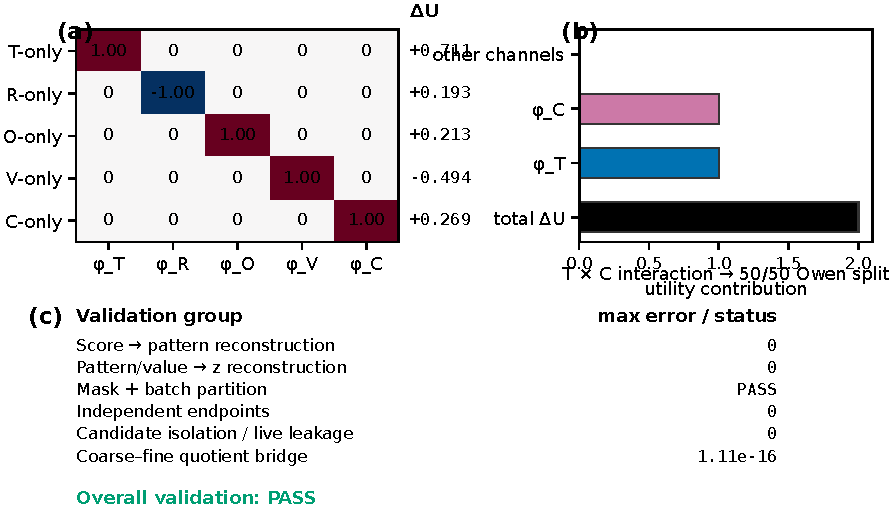
\includegraphics[width=\textwidth]{figures/Fig3.pdf}
\caption{\textbf{Controlled validation recovers known factors, interaction allocation, and transformer endpoint identities.}
(a) In five deterministic single-factor systems, the manipulated factor receives the full endpoint change: each row shows the recovery ratio $\phi_j/\Delta U_i$, with the raw injected $\Delta U_i$ given beside the row. The maximum attribution discrepancy is $1.11\times10^{-16}$.
(b) A pure $T\times C$ construction with $\Delta U\approx2$ yields the analytically expected Owen split $\phi_T\approx1$ and $\phi_C\approx1$, with $R,O,V=0$.
(c) In the randomly initialized two-layer TransformerLens validation model, independently measured intact effect, conditional effect, and conditional gain are $0.455046$, $-0.085684$, and $-0.540729$, respectively, and the corresponding FALI endpoint cells reproduce them exactly at recorded precision. Reconstruction, leakage, and model-level quotient residuals are zero at recorded precision.
These are implementation and controlled-ground-truth checks, not evidence that mixed FALI hybrids are unique natural model pathways.}
\label{fig:validation}
\end{figure*}
